\documentclass{LCSI_PhD}
\usepackage{macros}
\usepackage{hyperref}

\newcommand{\phdtitle}{Vers une am\'elioration des r\'esum\'es automatiques de textes}
\newcommand{\phdstudentname}{Aries Abdelkrime}
\newcommand{\advisorsname}{Pr. Zeggour Djamal Eddine, Pr. Hidouci Khaled Walid}
\newcommand{\teamname}{/}

\begin{document}
\headofpage

\begin{abstract}
In this report, we want to present our state of research advancement for the year 2014-2015. 
First, we will talk about summarization problems, such as the absence of corpora and NLP tools.
Then, we will present our system which is supposed to be language and domain independent. 
To test it, we participated in MultiLing'15 workshop (SIGDIAL'15 conference) in two tasks: single and multi-document summarization.
The system gives fair results, but it needs more improvement, especially when it comes to summary's coherence.
\end{abstract}

% Comment the following line if content is in French
%\selectlanguage{american}
%\selectlanguage{french}

\section{Introduction}

% Problem of huge information
With the considerable increase of information on the Internet, it has become very difficult to select relevant information.
The selection of the important information can be done using automatic text summarization. 
This is not the only benefit; it can, also, save time, ease the search, improve indexing, etc.
The resulted summary must be brief, relevant and coherent. 

%History
Automatic text summarization is not a new filed of research; many works have been done to improve this field. 
Recently, multilingual summarization has received the attention of the summarization community, such as Text Analysis Conference (TAC).
The TAC 2011 workshop included a task called ``MultiLing task", which aims to evaluate language-independent summarization algorithms on a variety of languages.
In 2013, this task became a separate workshop.
In MultiLing 2015\cite{15-giannakopoulos-al}, there were 12 participating systems, including ours. 
We were interested on two tasks: multilingual single document summarization and multilingual multi-document summarization.

\section{The problem}

Most work in the field of automatic text summary are based on extraction approaches.
The most relevant units (usually sentences) in the source text are extracted to form  a summary.
In the other hand, abstraction approaches are based on the generation of new sentences.
Due to the absence of effective NLP tools, this approach is too difficult.
Machine learning techniques are often used to improve the work of automatic summarization.
Their objective is to learn, from a corpus of documents, how to summarize a text.
The problem with these techniques is the absence of labeled training corpora.

Our objective is to create a system (method) which can be applied to any language and domain, yet it has to afford good summary.
Using extractive methods can be beneficial, this is why we proposed a method as a start \cite{13-aries-al}. 
This method has a lot to be ameliorated, from the preprocessing task and estimating hyper-parameters to fixing information redundancy and summary presentation.

\section{Carried work}

\subsection{System overview}

In our previous work \cite{13-aries-al}, our system used only two features which have the same nature (TF: uni-grams and bi-grams). 
When we add new features, this can affect the final result (summary).
Also, our clustering method lies on the clustering threshold which has to be estimated somehow. 
To handle multi-document summarization, we just fuse all documents in the same topic and consider them as one document.
%The only difference from single document summarization is the position feature which will be discussed later.
Figure \ref{fig:gnrl-arch} represents the general architecture of AllSummarizer\footnote{\url{https://github.com/kariminf/AllSummarizer}}.

\begin{figure}[h]
\centering
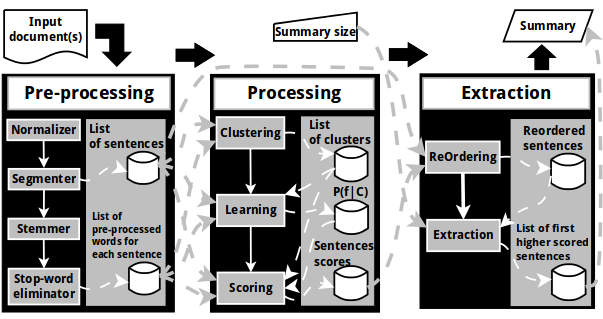
\includegraphics[width=9cm]{IMG/gnrl-arch.pdf}
\caption{General architecture of AllSummarizer.}
\label{fig:gnrl-arch}
\end{figure}

\subsubsection{Preprocessing}

This is the language-dependent part, which can be found in many information retrieval (IR) works. 
In our system, we are interested in four pre-processing tasks: Normalizer, Segmenter, Stemmer and Stop-Words eliminator.

\subsubsection{Topics clustering}

Each text contains many topics, where a topic is a set of sentences having some sort of relationship between each other.
To find the topics, we clustered similar sentences, where a sentence can belong to more than one cluster.
To calculate the similarity between two sentences, we used cosine similarity.
Then, we decide if two sentences are similar using a clustering threshold.

\subsubsection{Scoring function}

A summary is a short text that is supposed to represent most information in the source text, and cover most of its topics.
Therefore, we assume that a sentence $ s_i $ can be in the summary when it is most probable to represent all topics (clusters) $ c_j \in C $ using a set of features $ f_k \in F $.
We used a scoring function based on Na\"ive Bayes, assuming independence between different classes and different features (see equation\ref{eq:score}). 
\begin{equation}
\label{eq:score}
Score(s_i , c_j , f_k ) = 1 + \sum_{\phi \in s_i} {P(f_k=\phi | s_i \in c_j)}
\end{equation}
Where $ \phi $ is an observation of the feature $ f_k $ in the sentence $ s_i $.

The probability of the observation can be estimated from the clusters using the equation \ref{eq:likelihood}.
\begin{equation}
\label{eq:likelihood}
P_{f}(f = \phi | c_j) = \frac {|\phi \in c_j|}{\sum_{c_l \in C}{|\phi' \in c_l|}}
\end{equation}
Where $ f $ is a given feature.
$ \phi $ and $ \phi' $ are observations (categories) of the feature $ f $ .
$ C $ is the set of clusters.

\subsection{Statistical features}

We use 5 statistical features to score the sentences:
Unigram term frequency, 
Bigram term frequency,
Sentence position, and
Sentence length (Real length and preprocessed length)



\subsection{Summary extraction}
To extract sentences, we reorder them decreasingly using their scores. 
Then, we take the highest scored sentences as a summary. 
To reduce redundancy, each time we want to add a sentence to the summary, we compare it to the last added one. 
If they are similar, we don't add it. 
To compare them, we use cosine similarity and clustering threshold.

\subsection{Estimating summarization parameters}

The first parameter is the clustering threshold, which will lead to few huge clusters if it is small, and inversely.
To estimate it, eight measures have been used:
the median, the mean, the mode (lower and higher), the variance, $ sDn = \frac{\sum |s|}{|D| * n}$, 
$ Dsn = \frac{|D|}{n * \sum |s|}$,  $ Ds = \frac{|D|}{\sum |s|}$.
Where, $|s|$ is the number of different terms in a sentence $s$. 
$|D|$ is the number of different terms in the document $D$.
$n$ is the number of sentences in this document.

The second parameter is the features' set, which is the combination of at least one of the five features described previously. 
We want to know which features are useful and which are not for a given language.

To fix the problem of the clustering threshold and the set of features, we used the training sets provided by the MultiLing'15 workshop organizers.
For each document (or topic in multi-document), we generated summaries using the 8 measures of $ th $, and different combinations of the scoring features. 
Then, we calculated the average ROUGE-2 score for each language. 
The threshold measure and the set of features that maximize this average will be used as parameters for the trained language. 

\subsection{Experiments}

in our recent work \cite{15-aries-al}, we participated in MultiLing'15 workshop using all workshop's languages, either in single document or multi-document tasks.
To compare our system to others participated systems, we followed these steps (for every evaluation metric): 
\begin{itemize}
\item For each system, calculate the average scores of all used languages.
\item For our system, calculate the average scores of used languages by others. 
For example, BGU-SCE-M team uses Arabic, English and Hebrew; 
We calculate the average of scores of these languages for this system and ours.
\item Then, we calculate the relative improvement using the averages $ \frac{our system - other system}{other system} $.
\end{itemize}

Besides our system (AllSummarizer), there are two more systems which participated in all 38 languages (EXB and CCS) in single-document, and 4 systems that participated with all the 10 languages in multi-document. 
Our system outperforms the baseline system. 
it took 5th place out of 7 participants in single-document, and 7th place out of 10 participants in multi-documents. 
For more detail, see \cite{15-aries-al}.

\section{Prospects}

For future work, parameters must be estimated for each document based on statistical criteria, rather than for each language.
Also, we want to investigate the effect of the preprocessing step and the clustering methods on the resulted summaries.
Finally, readability remains a challenge for extractive methods, especially when we want to use a multilingual method. 
So, as a long term prospect, we want to find a way to reorder sentences and to reformulate them in a multilingual way.

\section{Conclusion}

To overcome the absence of labeled corpora and NLP tools, we proposed a language and domain independent summarization system. 
Our system looks for the different topics in the input text, and extract the sentences which represents most of them. 
This led us to new problems, which are how to estimate the hyper-parameters (clustering threshold and features set). 
To estimate them, we generated multiple summaries varying the threshold and the features, and fix the parameters for each language. 
But, this is not our purpose; we want to estimate them based on the document itself, regardless its language or its domain. 
Our system gives fair results in its relevancy. 
But, since it is based on extractive method, more care have to be given to the resulted text in term of readability.

\bibliographystyle{IEEEtran}
\bibliography{biblio}

\end{document}


